\documentclass[a4paper,11pt]{article} %ADD diffusion OR archiv for final versions
\usepackage[francais]{babel}
\usepackage[utf8]{inputenc}
\usepackage[T1]{fontenc}
\usepackage[margin=20mm,bindingoffset=5mm]{geometry}
\usepackage{mathtools}
\usepackage{amsfonts}
\usepackage{amssymb}
\usepackage{textcomp}
\usepackage{graphicx}
\usepackage[many]{tcolorbox}
\usepackage{epstopdf}
\usepackage{xcolor}
\usepackage{bm}
\usepackage{cases}
\usepackage{xspace}
\usepackage{lmodern}

%%% Macros simples
\newcommand{\pointmedian}{\fontfamily{cmr}\selectfont\textperiodcentered}

\newenvironment{encart}[1]{%
	\begin{tcolorbox}
		[
		breakable, enhanced jigsaw, % to break box over page
		arc = 1mm, % curvature
		title = \textbf{#1}, % title
		coltitle = white, % title font color
		colbacktitle = blue, % light-gray title
		colback = white, % white background
		colframe = blue % dark frame
		]
}{		
	\end{tcolorbox}
}

\title{Mise en perspective didactique d'un projet de recherche}
\author{Tamara Bardon-Brun}
\date{Session 2022}

\begin{document}
	\label{key}
	\maketitle
	
	\section{Parcours universitaire}
	\subsection{\'{E}tudes}
	\begin{itemize}
		\item 2012--2015 : Licence de Physique Fondamentale à l'Université de Lille
		\item 2015--2016 : $1^\text{ère}$ année du master de Physique Fondamentale à l'Université Pierre et Marie Curie
		\item 2016--2017 : $2^\text{nde}$ année du master International Center of Fundamental Physics parcours Physique Quantique à l'\'{E}cole Normale Supérieure de Paris
		\item 2017--2020 : Thèse au sein du Laboratoire Kastler Brossel sous la direction de Nicolas Cherroret, intitulée \og Propagation de la lumière en milieu complexe : effet Hall de spin optique en présence de désordre et force de Casimir en milieu Kerr\fg{}, soutenue le 13 Janvier 2021
		\item 2021--2022 : Préparation de l'agrégation de Physique-Chimie option Physique au centre de Montrouge
	\end{itemize}
	
	\subsection{Enseignements, vulgarisation et autres activités}
	\begin{itemize}
		\item Participation au French Physicists' Tournament :
		\subitem 2016 : participation en tant que membre de l'équipe de Sorbonne Université
		\subitem 2018--2020 : encadrement de l'équipe de Sorbonne Université
		\subitem 2021--2022 : participation à l'équipe d'organisation du tournoi \\
		\item Monitorat à Sorbonne Université (3 ans) :
		\subitem Encadrement de TP d'optique en L3
		\subitem Chargée de TD en physique du mouvement en L2 \\
		\item Membre de CurieOsity, association des étudiant\pointmedian es de physique de Sorbonne Université :
		\subitem Organisation de conférences et de rencontres avec des chercheurs et des chercheuses
		\subitem Tutorat de physique\\
		\item Participation à la Fête de la science avec le laboratoire Kastler Brossel (2017--2020)
	\end{itemize}

	
	\section{Travail de recherche}
	\subsection{Motivations}
	Au cours du XXe siècle, le développement de la physique quantique a amené de nombreuses avancées dans la compréhension de la matière en permettant de mieux appréhender sa structure et le comportement de ses composants. Cela a provoqué l'essor de nombreux domaines de la matière condensée tels que la physique de semi-conducteurs, la supraconductivité, etc. De plus, depuis les années 90, l'amélioration des méthodes de refroidissement et de piégeage d'atomes permettent l'étude expérimentale de plus en plus poussée de systèmes quantiques. Ces systèmes d'atomes froids peuvent être manipulés avec une grande précision, nous permettant de simuler des phénomènes existant au c\oe ur de la matière en contrôlant un maximum de paramètres. Cependant, la nécessité de refroidir grandement ces systèmes pour voir apparaître un comportement quantique est une contrainte expérimentale très forte. Plus récemment, au début du XXIe siècle, s'est alors développée l'idée d'utiliser de la lumière pour reproduire de telles simulations. L'étude de tels systèmes optiques est également intéressante car la lumière est ici traitée de manière totalement classique or les phénomènes étudiés reposent pour la matière sur son aspect quantique.\\
	
	Lors de ma thèse, j'ai étudié analytiquement des cas de propagation de la lumière dans des milieux dits complexes où nous avons retrouvé des analogues optiques à deux phénomènes : l'effet Hall de spin et l'effet Casimir critique. Dans ce dossier, je vais présenter plus particulièrement mon travail sur l'effet Hall de spin optique dans un milieu désordonné. L'étude de ce phénomène amène notamment à s'intéresser à la question du spin d'un faisceau lumineux et à la notion de couplage spin-orbite en optique qui est un domaine récent de la physique.\\
	
	Afin de commenter les résultats de ma thèse sur l'effet Hall de spin optique en désordre transverse, nous commencerons par introduire rapidement les effets de couplage spin-orbite de la matière à travers l'exemple de l'effet Hall de spin. Nous introduirons ensuite des éléments de propagation de la lumière au sein de milieux inhomogènes et présenterons l'émergence dans de tels milieux d'effets analogues à des effets de couplage spin-orbite. Enfin, nous discuterons plus précisément le cas d'un milieu désordonné.
	
	
	\subsection{Effet de Hall de spin -- couplage spin-orbite dans la matière}
	
	\begin{figure}[h]
		\centering
		\begin{minipage}[c]{0.85\linewidth}
			\centering
			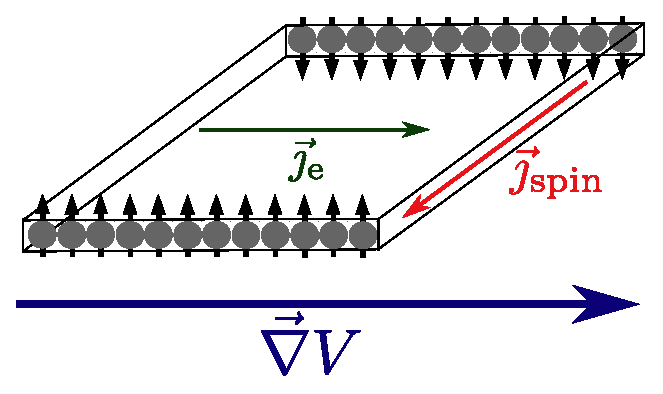
\includegraphics[width=0.5\linewidth]{./Illustrations/SHE_electrons.eps}
			\caption{Illustration de l'effet Hall de spin dans un échantillon 2D métallique soumis à un gradient de potentiel électrique.}
			\label{fig:spin-Hall-effect}
		\end{minipage}
	\end{figure}
	
	L'effet Hall est un effet aujourd'hui bien connu en physique (voir activité pédagogique 1) : un échantillon soumis à champ magnétique et traversé d'un courant électrique voit apparaître une accumulation de charges sur ses bords. Cet effet s'explique par le couplage entre les charges électriques en mouvement et le champ magnétique, les électrons étant alors déviés par la force de Lorentz. Il existe un effet analogue faisant intervenir le couplage entre le champ électrique (utilisé pour générer le courant) et le spin porté par les électrons : ce phénomène est appelé effet Hall de spin. Il s'agit d'un effet de couplage spin-orbite que nous allons présenter.\\ 
	
	\begin{encart}{Activité pédagogique 1 : étude de l'effet Hall classique}
		\textbf{Contexte :}
		\begin{itemize}
			\item niveau : CPGE $ 2^\text{ème} $ année --- filière PC
			\item place dans la progression : partie \'Electromagnétisme -- chapitre Conduction électrique
		\end{itemize}
		\vspace{0.5cm}
		
		\textbf{Objectifs pédagogiques :}
		\begin{itemize}
			\item exploiter les connaissances acquises dans les chapitres précédents pour obtenir une description classique de l'effet Hall
			\item caractériser la tension de Hall
			\item en connaître des applications (mesure de champ magnétique notamment)
		\end{itemize}
		\vspace{0.5cm}
		
		\textbf{Déroulement résumé de l'activité :}\\
		I -- Description théorique (séance de cours) :
		\begin{itemize}
			\item Introduction des résultats historiques de Hall $ \Rightarrow $ caractéristiques de la tension de Hall
			\item Présentation du système
			\item Déviation des électrons par le champ magnétique : accumulation de charges sur les bords de l'échantillon
			\item Apparition d'un champ électrique s'opposant à la force magnétique
			\item \'Etude du régime stationnaire et obtention de l'expression de la tension de Hall.
		\end{itemize}
		\vspace{0.5cm}
		
		II -- Observation expérimentale (séance de TP) :\\
		En utilisant des échantillons semi-conducteurs traversés par un courant et placés dans un champ magnétique, il est possible de mesurer la tension de Hall.\\
		Objectifs de la séance :
		\begin{itemize}
			\item Observer la proportionnalité de $ V_H $ avec $ I $ et $ B $
			\item Déduire le signe des porteurs de charge du sens de la différence de potentiel
			\item pour aller plus loin : remonter à la densité des porteurs de charge
		\end{itemize}
		
		\vspace{0.5cm}
		III -- Ouverture :\\
		La notion de spin était également vu par les élèves, il serait possible de leur présenter qualitativement l'effet Hall de spin en faisant une analogie entre charge électrique dans un champ magnétique et moment magnétique de spin dans un champ électrique. Cela permettrait de leur présenter un exemple original de phénomène faisait intervenir la notion de spin.
	\end{encart}
	
	L'effet Hall de spin apparaît dans un échantillon bidimensionnel d'un semi-conducteur soumis à une différence de potentiel électrique $\vec{\nabla} V$. L'hamiltonien d'un électron dans ce système est alors donné par l'expression :
	\begin{equation*}
		\label{exp_hamiltonien_SHE}
		H = \frac{\vec{p}^{\, 2}}{2m_e} + q_e V(\vec{r}) + \mathcal{A}_\textup{SO} \, (\vec{p} \wedge \! \vec{\nabla} V) \cdot \vec{S}
	\end{equation*}
	où $ \vec{p} $ est l'impulsion de l'électron et $ \vec{S} $ son spin. Nous avons introduit ici le coefficient de couplage spin-orbite $ \mathcal{A}_\textup{SO} $ qui dépend des propriétés de symétrie du matériau considéré.\\
	
	En passant par les équations d'Hamilton, il est possible de décrire la trajectoire semi-classique des électrons. Nous obtenons alors les équations du mouvement :
	\begin{align}
		& \frac{d\vec{r}}{dt} = \frac{\vec{p}}{m} - \mathcal{A}_{SO} \vec{S} \wedge \vec{\nabla} V \label{eq_mvt_SHE_r} \\
		& \frac{d \vec{p}}{dt} = - q_e \vec{\nabla} V \label{eq_mvt_SHE_p}
	\end{align}
	où nous voyons ici apparaître un terme supplémentaire (par rapport à la trajectoire attendue pour un électrons soumis à un champ électrique) dans l'équation \eqref{eq_mvt_SHE_r} lié au couplage spin-orbite. L'impulsion, elle, n'est pas modifiée : on parle alors de décalage du faisceau d'électrons. Celui-ci a pour caractéristique d'être perpendiculaire au gradient de potentiel et à la direction du spin : c'est un décalage transverse. Il est également proportionnel à la différence de potentiel électrique et son signe dépend de l'orientation du spin.
	
	
	\subsection{Effet de couplage spin-orbite de la lumière en milieux inhomogènes}
	De telles considérations sur le couplage spin-orbite ont été initialement étudiés uniquement pour la matière. Pourtant ces effets existent aussi pour la lumière, cependant leur contribution se limitent alors à des échelles inférieures à celle de la longueur d'onde, leur étude ne s'est donc développée que récemment, en particulier avec l'émergence de la nanophotonique. Cette description s'avère cependant très riche et permet notamment de mieux comprendre des phénomènes qui étaient déjà connus tels que l'effet Imbert--Fedorov ou l'effet Magnus optique, ce que nous discuterons rapidement dans cette partie.
	
	\subsubsection{Propagation en milieu inhomogène -- cas de l'approximation paraxiale}
	Lorsque l'on considère un milieu diélectrique (non magnétique), la propagation d'un faisceau lumineux en son sein est caractérisée par sa permittivité relative $ \epsilon $ (que l'on suppose ici réelle) ou de manière équivalente par son indice optique $ n = \sqrt{\epsilon} $. Si l'on considère un milieu homogène, la lumière s'y propage en ligne droite et l'influence du milieu se résume finalement à la modification de la longueur d'onde : $ \lambda_\text{milieu} = \lambda_\text{vide} / n $. Cependant, dans le cas général, un faisceau lumineux rencontre des variations d'indice d'optique au cours de sa propagation. Il est donc important de savoir décrire l'influence de cette inhomogénéité.\\
	Afin de décrire l'évolution d'un faisceau lumineux, on étudie la trajectoire de son centroïde que l'on notera $ \vec{R} $ et qui est le barycentre du faisceau pondéré par la densité d'énergie du champ électromagnétique.\\
	
	
	\begin{encart}{Activité pédagogique 2 : réfraction à une interface -- Loi de Snell-Descartes}
		\textbf{Contexte :}
		\begin{itemize}
			\item niveau : $ 2^\textup{nde} $ générale
			\item place dans la progression : partie Ondes et signaux -- Chapitre Vision et image
		\end{itemize}
		\vspace{0.5cm}
		
		\textbf{Objectifs pédagogiques :}
		\begin{itemize}
			\item connaître la loi de Snell--Descartes
			\item observer et caractériser la réfraction à une interface
			\item obtenir expérimentalement l'indice optique d'un milieu
		\end{itemize}
		\vspace{0.5cm}
		
		\textbf{Résumé de l'activité :}\\
		Lors de cette activité, les élèves vont observer la réfraction de la lumière passant dans un cuve d'eau. Par la mesure de l'angle réfracté pour différents angles d'incidence, on remonte à l'indice optique du plexiglas en utilisant la loi de Snell--Descartes vu en cours précédemment. De plus, en dissolvant ensuite du sucre dans la cuve, les élèves pourront directement jouer sur l'indice optique de la solution et observer le changement sur l'angle réfracté.\\
		
		\textbf{Déroulé de l'activité :}
		On dispose d'une lampe avec un embout permettant de générer un faisceau lumineux fin, de plusieurs cuves d'eau et de sucre.
		\begin{itemize}
			\item envoyer le faisceau lumineux en incidence normale sur la cuve : on n'observe pas de réfraction.
			\item augmenter légèrement l'angle d'incidence (on observe ici l'interface air-eau) : observer que l'angle au sein du milieu est différent de l'angle d'incidence.
			\item pour différents angles d'incidence, mesurer l'angle réfracté.
			\item vérifier que les sinus des angles suivent bien une relation de proportionnalité, en déduire la valeur de l'indice optique $ n $ de l'eau (en considérant $ n_{air} = 1 $).
			\item \textit{(ici on pourra éventuellement discuter de l'influence de la paroi de la cuve si certains groupes avancent plus rapidement)}
			\item dans une autre cuve, dissoudre une bonne quantité de sucre
			\item pour un angle d'incidence déjà mesuré dans la cuve d'eau non-sucrée relever la nouvelle valeur de l'angle réfracté
			\item en déduire l'influence de la dissolution du sucre sur l'indice optique de la solution
			\item \textit{démonstration professeur\pointmedian e : dans une grande cuve ajouter du sucre au fond sans mélanger, envoyer un faisceau laser dans le milieu, l'inhomogénéité de concentration provoque une déviation du faisceau} 
		\end{itemize}
		
	\end{encart}

	Le cas le plus simple d'inhomogénéité que l'on peut considérer est le cas d'une interface entre deux milieux d'indice optique différent (voir activité pédagogique 2). La description d'un milieu inhomogène continu est alors obtenue en considérant le gradient d'indice optique comme une succession d'interfaces entre deux indices $ n_i $ et $ n_i + dn_i $. L'inhomogénéité du milieu résulte alors en une courbure du faisceau lumineux qui s'y propage. C'est ce qui explique l'apparition des mirages (voir activité pédagogique 3).\\
	
	\begin{encart}{Activité pédagogique 3 : description qualitative d'un mirage}
		\textbf{Contexte :}
		\begin{itemize}
			\item niveau : $ 2^\text{nde} $ générale
			\item place dans la progression : partie Ondes et signaux -- Chapitre Vision et image  
		\end{itemize}
		\vspace{0.5cm}
		
		\textbf{Objectifs pédagogiques :}
		\begin{itemize}
			\item proposer un modèle permettant d'expliquer le phénomène des mirages
		\end{itemize}
		\vspace{0.5cm}
		
		\textbf{Résumé de l'activité :}
		L'objectif est ici de discuter avec les élèves et de les amener à exploiter ce qu'ils et elles ont vu précédemment pour décrire un phénomène optique plus complexe qu'est le mirage.\\
		
		\textbf{Déroulement de l'activité :}
		\begin{itemize}
			\item Question ouverte posée à la classe : \og qu'est-ce qu'un mirage ?\fg{}
			\item Amener les élèves à s'interroger sur les conditions de formation du mirage
			\item Présentation du phénomène de courbure (photo, vidéo et/ou démonstration devant la classe)
			\item Discussion de la variation de l'indice optique de l'air en fonction de la température
			\item Construction qualitative de la trajectoire du faisceau lumineux pour un mirage.
		\end{itemize}
		
	\end{encart}
	
	Afin d'étudier la propagation dans un milieu inhomogène, un cadre intéressant est celui de l'approximation paraxiale qui permet de décrire les faisceaux lumineux se propageant avec une direction proche de l'axe optique du milieu. Cet axe, que nous appellerons $ z $ dans toute la suite, est une direction selon laquelle la variation d'indice optique est négligeable. Nous écrivons alors la permittivité sous la forme :
	\begin{equation*}
		\epsilon(\vec{r}) \simeq \epsilon(x,y) = \bar{\epsilon} + \delta \epsilon(x,y) \; .
	\end{equation*}
	La description de la propagation lumineuse se fait par l'étude de l'évolution du champ électrique. Dans le cadre de l'approximation paraxiale, la composante longitudinale (selon $ z $) est négligée, ce qui nous amène à une description scalaire de la lumière. Cela est valide si l'enveloppe du champ électrique varie peu par rapport à la longueur caractéristique de variation de $\delta \epsilon (x,y)$ et revient à considérer l'hypothèse : 
	\begin{equation}
		\label{hyp_var_epsilon}
		\lambda \left| \frac{\vec{\nabla}\epsilon(x,y)}{\bar{\epsilon}} \right| \ll 1 \; \text{ ou de manière équivalente : } \; \lambda \left| \frac{\vec{\nabla}n(x,y)}{\bar{n}} \right| \ll 1 .
	\end{equation}
	
%	\begin{figure}[h]
%		\centering
%		\begin{minipage}[c]{0.85\linewidth}
%			\centering
%			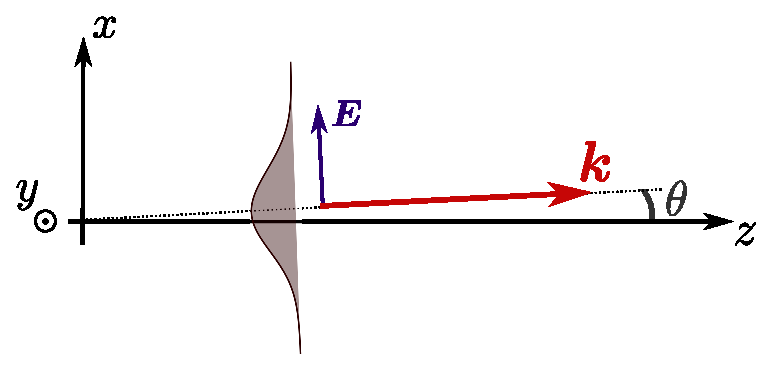
\includegraphics[width=0.65\linewidth]{./Illustrations/schema_paraxial}
%			\caption{Dans l'approximation paraxiale, nous étudions des faisceaux suffisamment collimatés, dont la direction de propagation $ \vec{k} $ est faiblement inclinée par rapport à un axe optique $ z $ ($ \theta \ll 1 $) et dont la variation de l'enveloppe est suffisamment molle.}
%			\label{fig:schema_paraxial}
%		\end{minipage}
%	\end{figure}
	
	Ce cadre permet de décrire la déviation du faisceau dans le plan de propagation sous l'effet d'une variation de la permittivité du milieu et amène à une bonne description de la trajectoire d'un faisceau lumineux à l'échelle macroscopique. Cependant, à ce stade, nous ne pouvons pas décrire les effets de couplage spin-orbite. Ceux-ci sont en effet liés à l'aspect vectoriel de la lumière. Nous allons donc à présent nous pencher sur les premières corrections à l'approximation paraxiale.
	
	\subsubsection{Au delà de l'approximation paraxiale : effet de couplage spin-orbite optique}
	
	Si l'on s'intéresse de plus près à la réflexion à une interface, en plus de la déviation du faisceau dans le plan incident, il existe également un décalage transverse du faisceau dépendant de la polarisation du faisceau : il s'agit de l'effet Imbert--Fedorov (évoqué pour la première fois en 1955 par Fedorov et mis en évidence en 1972 par Imbert). Ce décalage est de l'ordre de
	\begin{equation*}
		\delta R \sim - \frac{\sigma}{k}
	\end{equation*}
	où $ \sigma $ est l'hélicité du faisceau qui caractérise son état de polarisation. Celle-ci varie entre 0 pour un polarisation rectiligne et $\pm 1 $ pour une polarisation circulaire, les valeurs intermédiaires caractérisant une polarisation elliptique. La question est à présent de généraliser ce résultat décrivant le cas d'une interface aux milieux inhomogènes. Si l'on reprend les calculs de la propagation du champ électrique en prenant en compte les termes d'ordre $ \lambda | \vec{\nabla}n | / n \ll 1$, la trajectoire du faisceau lumineux s'écrit alors :
	\begin{equation}
		\frac{d \vec{R}}{dz} = \frac{\vec{k}}{k} - \frac{\sigma}{k} \left[ \frac{\vec{k}}{k} \wedge \vec{\nabla}(\ln n) \right] \; .
	\end{equation}
	Ce décalage a été étudié pour la première fois en 1992 par Liberman et Zel'Dovich qui l'ont interprété comme un effet Magnus de la lumière. En effet, une analogie apparaît avec la déviation d'un objet en rotation au sein d'un fluide en écoulement. Cependant, il est également possible de comparer cette trajectoire avec celle de l'effet Hall de spin donnée par l'équation \eqref{eq_mvt_SHE_r}, d'où la notion de couplage spin-orbite de la lumière. Nous voyons alors plusieurs éléments intéressants apparaître. Tout d'abord, nous pouvons remarquer que le gradient d'indice optique du milieu joue pour la lumière le rôle du gradient de potentiel. Nous voyons alors que si dans le cas de l'effet Hall de spin, le couplage spin-orbite était lié au matériau considéré par le coefficient $ \mathcal{A}_\textup{SO} $, pour la lumière, le terme qui apparaît ici ne dépend pas explicitement du milieu considéré. Cela fait de la lumière un très bon candidat pour étudier ces effets. Enfin, nous voyons ici que le terme $ \sigma \vec{k} /k $ s'identifie au spin de l'électron dans l'équation \eqref{eq_mvt_SHE_r}, il est donc possible de faire un lien direct entre la polarisation de la lumière et son spin. En fait, on peut même définir de manière générale la notion de moment cinétique pour un faisceau lumineux, c'est ce que nous allons présenter rapidement.
	
	\subsubsection{Notion de moment cinétique de la lumière}
	Tout comme pour les particules matérielles, il est possible de définir une impulsion locale du faisceau lumineux. Celle-ci est donnée (pour une lumière monochromatique) par 
	\begin{equation*}
		\vec{p} = \frac{\epsilon_0}{2} \vec{E}(\vec{r}, \omega) \wedge \vec{B}(\vec{r}, \omega) \; .
	\end{equation*}
	Nous pouvons alors écrire le moment cinétique total local du faisceau :
	\begin{equation*}
		\vec{\jmath} \, (\vec{r}) = \vec{r} \wedge \vec{p}(\vec{r}) \; .
	\end{equation*}
	
	Dans le cadre de l'approximation paraxiale, le moment cinétique total du faisceau est donné par l'expression
	\begin{equation}
		\vec{J}(z) = \frac{\epsilon_0}{2 i \omega} \int dx dy \left[ E_i^* (\vec{r} \wedge \vec{\nabla}) E_i + \vec{E}^* \wedge \vec{E} \right] \; ,
	\end{equation}
	où nous avons utilisé la notation d'Einstein. Nous voyons alors apparaître deux contributions différentes.\\
	
	La première contribution dépend de la variation du champ électrique, il s'agit du moment cinétique orbital de la lumière. Elle peut être due à une déformation du front d'onde, c'est ce que l'on appelle le moment cinétique orbital intrinsèque représenté sur la figure \ref{fig:moments_angulaires}(a), ou bien à la trajectoire du faisceau, c'est ce que l'on appelle le moment cinétique orbital extrinsèque représenté sur la figure \ref{fig:moments_angulaires}(b).\\	
	
	La deuxième contribution est uniquement liée à la valeur locale du champ électrique, c'est celle que l'on va interpréter comme un moment cinétique de spin représenté sur la figure \ref{fig:moments_angulaires}(c). Dans le cas d'un faisceau collimaté, celui-ci va être donné par l'expression :
		\begin{equation*}
			\vec{S} = \frac{\epsilon_0 I}{\omega} \; \frac{\sigma \vec{k}}{k}
		\end{equation*}
	où nous avons introduit l'intensité $ I $ du faisceau et son hélicité $ \sigma $. Nous retrouvons ainsi que le spin d'un faisceau lumineux est directement lié à la polarisation de la lumière, un spin non-nul correspondant alors à une polarisation tournante du faisceau lumineux. Notons ici que l'on est toujours dans une description classique de la lumière, contrairement au spin des électrons, utilisé dans l'équation \eqref{exp_hamiltonien_SHE}, qui est une notion totalement non-classique puisqu'elle est quantique et relativiste.	
	
	
	
	\begin{figure}[h]
		\centering
		\begin{minipage}[c]{0.9\linewidth}
			\centering
			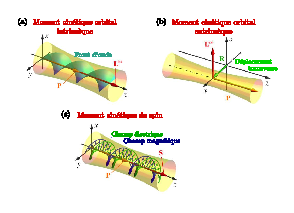
\includegraphics[width=0.8\linewidth]{./Illustrations/moments_angulaires}
			\caption{Illustrations des différents moments cinétiques de la lumière,tirées de l'article de Bliokh, Rodriguez-Fortuño, Nori et Zayats. (a) Le moment cinétique orbital intrinsèque, lié à une variation de la phase du champ ; (b) le moment cinétique orbital extrinsèque, lié à un déplacement du faisceau lumineux par rapport à une origine ; (c) le spin du faisceau lumineux, lié à la rotation des champs électrique et magnétique. Ici, la notation $ \vec{P} $ correspond à l'impulsion moyenne du faisceau.}
			\label{fig:moments_angulaires}
		\end{minipage}
	\end{figure}
	
%	\begin{figure}[h]
%		\centering
%		\begin{minipage}[c]{0.85\linewidth}
%			\centering
%			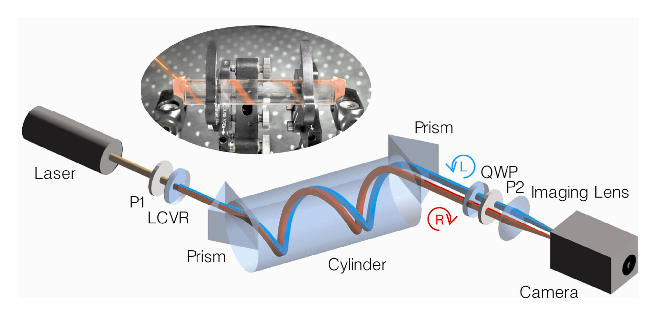
\includegraphics[width=0.9\linewidth]{./Illustrations/Bliokh_mesure_SHE-light-1.eps}
%			\caption{Figures tirées de l'article de Bliokh, Niv, Kleiner et Hasman. Schéma du montage expérimental utilisé pour mesurer les décalages transverses liés à l'effet Hall de spin optique : un faisceau laser polarisé circulairement est envoyé en incidence rasante sous la surface d'un cylindre au sein duquel il suit une trajectoire hélicoïdale. La position du faisceau à la sortie est mesurée à l'aide du caméra. L'angle d'incidence du laser permet de contrôler le nombre de tours effectués par le faisceau au sein du cylindre.}
%			\label{fig:mesure_SHE_light}
%		\end{minipage}
%	\end{figure}
	
	\subsection{Effet Hall de spin optique en désordre transverse}
	Les effets de couplage spin-orbite de la lumière que nous avons présentés précédemment ont été étudiés dans des systèmes où la variation d'indice optique est connue. Au cours de ma thèse, je me suis intéressée à l'étude de tels effets au sein de milieux désordonnés. Il s'agit à notre connaissance des premières investigations à ce sujet.\\
	Avant de discuter les résultats obtenus, nous allons commencer par rapidement présenter des éléments de description de la propagation en milieux désordonnés, puis nous introduirons le système considéré.
	
	\subsubsection{Propagation dans un système désordonné}
	
	Les milieux dits désordonnés sont des milieux très inhomogènes où l'indice optique varie de manière aléatoire. Cela va correspondre par exemple à des poudres, du verre dépoli ou des solutions contenant des particules en suspension. Lorsqu'un faisceau lumineux se propage dans de tels milieux, nous pouvons observer différents phénomènes illustrés sur la figure \ref{fig:diffusion_desordre_3D}. Si l'on observe le comportement de la lumière au sein du milieu (comme montré sur la figure \ref{fig:diffusion_desordre_3D}(b)), nous pouvons tout d'abord décrire deux  composantes différentes :
	\begin{itemize}
		\item le faisceau balistique qui décrit la trajectoire que l'on attendrait en absence de désordre. Son intensité décroit de manière exponentielle lors de la propagation dans le milieu sur une longueur caractéristique $\ell$.
		\item le halo diffusif qui lui apparaît autour du faisceau balistique au cours de la propagation.
	\end{itemize}
	Ces comportements sont dus à la diffusion de la lumière de la lumière sur les petits obstacles qui sont à l'origine de l'inhomogénéité du milieu. La longueur caractéristique $\ell$ de la diffusion est alors la distance moyenne entre deux processus de diffusion appelée libre parcours moyen. Si on considère une lumière cohérente, les composantes du halo diffusif se propageant dans différentes directions vont interférer, on voit alors apparaître un profil d'intensité désordonné appelée \textit{speckle}, avec des tâches lumineuses entourées de zones plus sombres comme présenté sur la figure \ref{fig:diffusion_desordre_3D}(a).\\
	
	\begin{figure}[h]
		\centering
		\begin{minipage}[c]{0.85\linewidth}
			\centering
			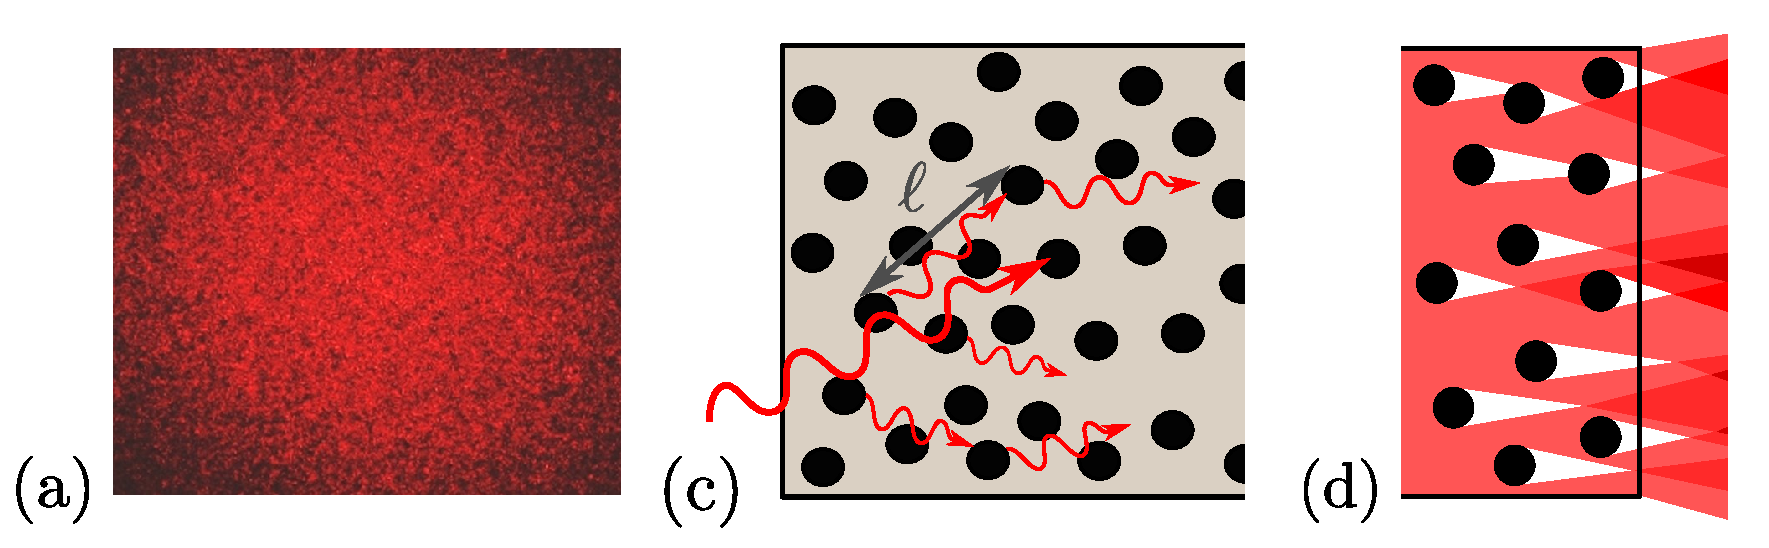
\includegraphics[width=0.85\linewidth]{./Illustrations/figure_scatt.eps} \\
			(b) \hspace{0.1cm} 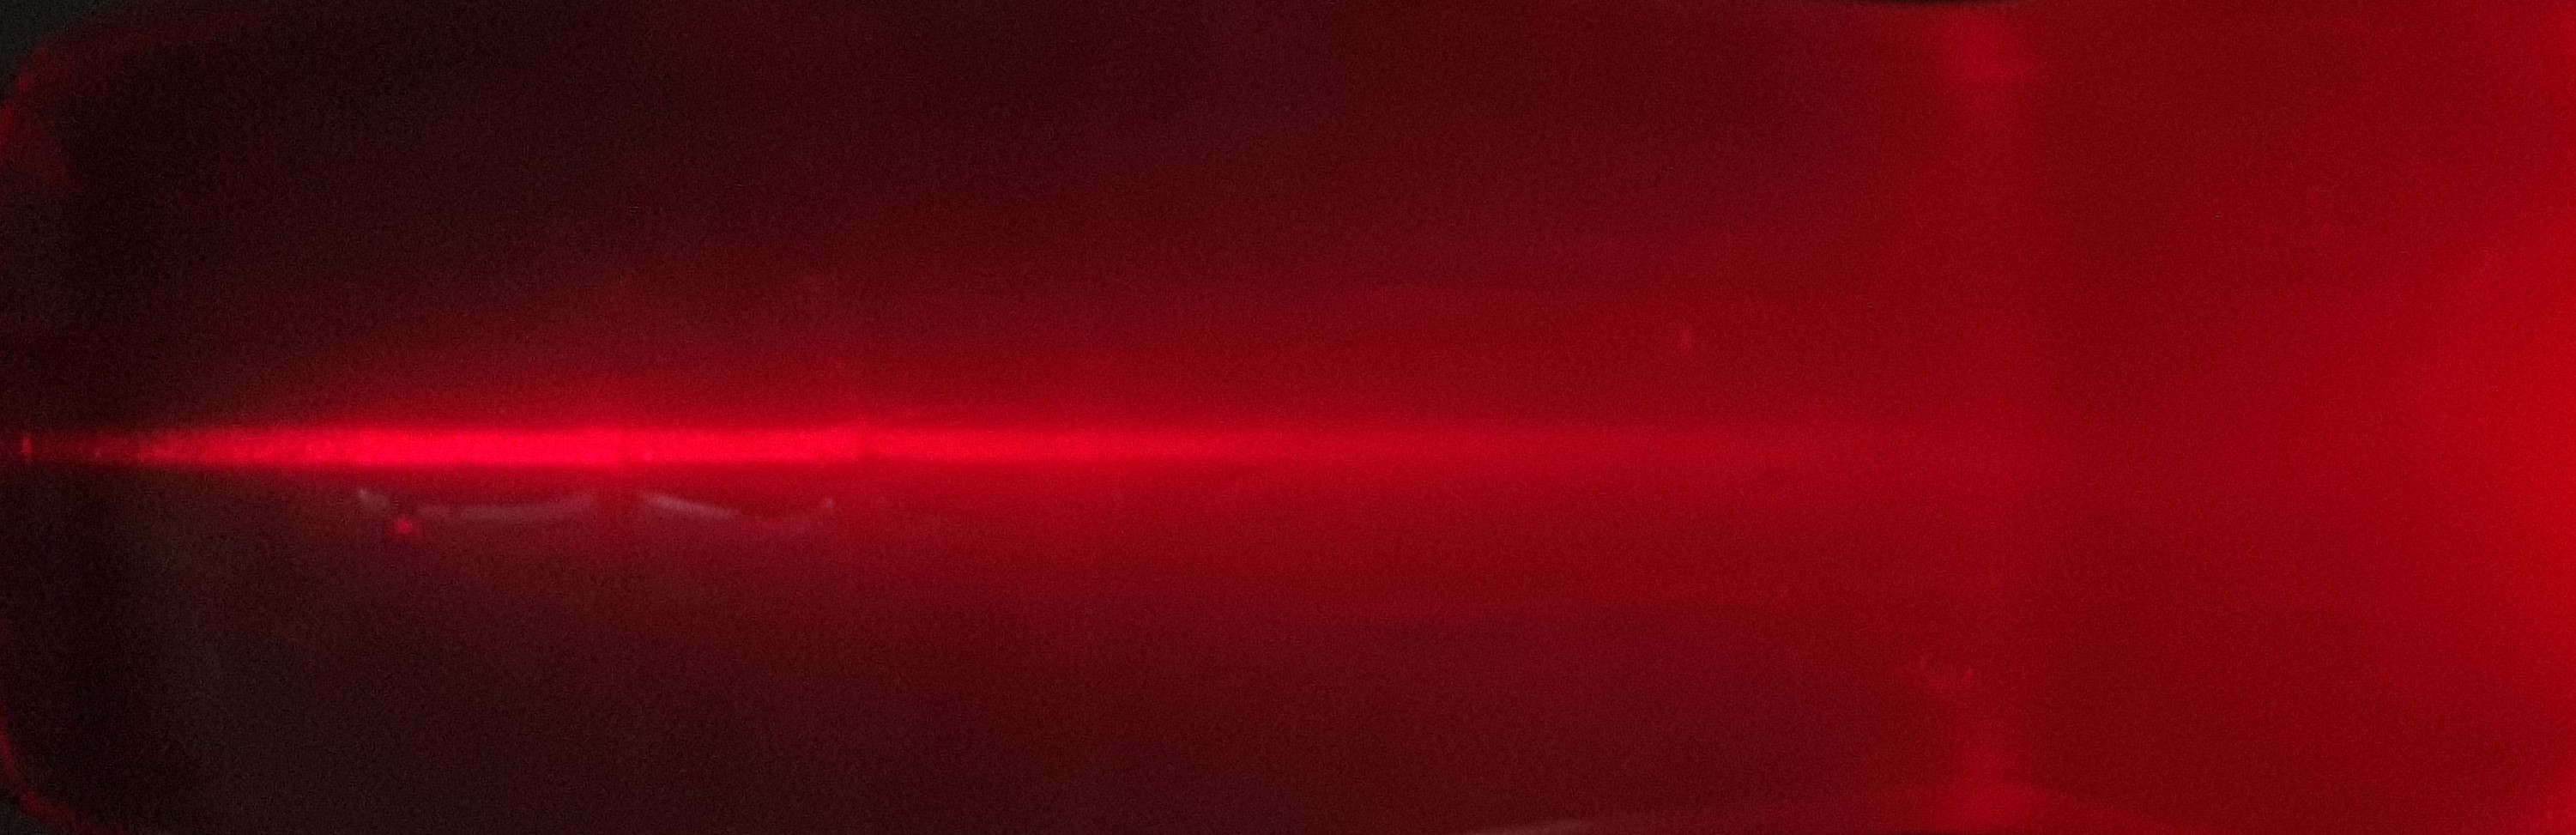
\includegraphics[width=0.8\linewidth]{./Illustrations/Photo_diff_desordre_3D}
			\caption{(a) Photo d'un speckle produit par un faisceau laser après propagation au travers d'un morceau de plastique rugueux. (b) Photo du phénomène de diffusion multiple dans un milieu diffusant (ici de l'eau contenant un peu de maïzena en suspension). (c) Schéma de la diffusion de la lumière se propageant à travers une distribution aléatoire de diffuseurs. (d) Schéma de la lumière diffusée à la sortie du milieu.}
			\label{fig:diffusion_desordre_3D}
		\end{minipage}
	\end{figure}	
	
	Une description analytique complète de ce problème est presque impossible. Afin de décrire les phénomènes de propagation dans un milieu désordonné, nous nous basons sur une approche statistique. Nous pouvons alors obtenir l'expression du champ électrique moyenné sur différentes réalisations du désordre. Ce champ moyen permet de décrire la propagation du faisceau balistique qui est la composante qui nous intéresse ici.
	
	
	\subsubsection{Présentation du système : désordre transverse}
	
	\begin{figure}[h]
		\centering
		\begin{minipage}[c]{0.85\linewidth}
			\centering
			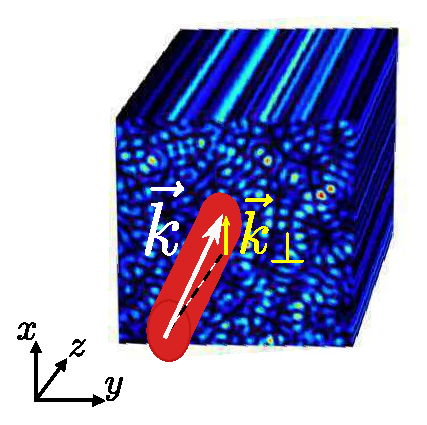
\includegraphics[width=0.35\linewidth]{./Illustrations/2+1disorder.eps}
			\caption{Illustration d'un milieu désordonné dans le plan transverse $ (x,y) $ et homogène selon l'axe optique $ z $, sur lequel est envoyé un faisceau lumineux collimaté \textit{tilté}, de vecteur d'onde transverse $ \vec{k}_\perp $ selon $ \vec{e}_x $.}
			\label{fig:systeme_desordre_transverse}
		\end{minipage}
	\end{figure}

	Afin de voir apparaître des effets de couplage spin-orbite, il est nécessaire d'avoir une certaine anisotropie du système car s'il n'existe aucune direction privilégiée (ou plus précisément, si on ne peut pas définir un axe optique), il ne peut pas y avoir apparition d'un décalage transverse (dont la direction est définie par rapport au plan contenant le faisceau et l'axe optique). Ici, nous avons choisi de considérer le cas où la permittivité est parfaitement homogène selon l'axe $ z $ mais varie aléatoirement dans le plan $ (x,y) $, comme représenté sur la figure \ref{fig:systeme_desordre_transverse}, c'est ce que l'on nomme désordre transverse. Nous allons y décrire la propagation d'un faisceau gaussien collimaté arrivant avec un léger angle dans le plan $ (x,z) $ et dont la polarisation initiale est décrite par le vecteur $ \vec{\varepsilon} $ (réel pour une polarisation rectiligne et complexe pour une polarisation elliptique). Nous nous intéressons ici à la trajectoire du faisceau dans le plan transverse $ (x,y) $, nous considérons ainsi un système à 2 dimension, tandis que la coordonnée $ z $ joue ici le rôle d'un temps (ce qui apparaît explicitement lorsque l'on écrit les équations de propagation).\\
	
	En première approximation, c'est-à-dire dans l'approximation paraxiale, on obtient, comme attendu pour le faisceau balistique, une trajectoire rectiligne caractérisée par le vecteur d'onde transverse $ \vec{k}_\perp $. De plus, l'intensité du faisceau décroit exponentiellement avec un temps caractéristique de diffusion $ z_d $ qui dépend des caractéristiques du désordre. Le libre parcours moyen est alors donné par $ \ell = k_\perp/k \; z_d $\\
	
	\subsubsection{Décalage transverse du faisceau}
	
	Afin de décrire les effets de couplage spin-orbite, tout comme dans les cas présentés dans la partie précédente, nous allons prendre en compte les premières corrections liées à l'aspect vectoriel du champ électrique. Nous nous intéressons ici plus particulièrement au faisceau balistique, décrit par le champ électrique moyen. L'étude de cette configuration est notamment intéressante car il n'est pas évident de savoir a priori si le décalage lié au couplage spin-orbite survit au moyennage sur le désordre.\\
	
	Après l'obtention de l'expression du champ moyen dans le désordre transverse, nous arrivons à l'expression de la trajectoire du centre du faisceau :
	\begin{equation*}
		\vec{R}_\perp (z) = \frac{\vec{k}_\perp}{k} z - \frac{\sigma}{k_\perp} \left[ 1 - \frac{1}{\cosh (z/z_\text{\tiny SH})} \right] \vec{e}_y \; ,
	\end{equation*}
	où nous avons introduit un nouveau temps caractéristique $ z_\text{{\tiny SH}} = 2 (k/k_0)^2 z_s  $ . Nous voyons ici deux termes, le premier correspond à la propagation balistique attendue sans la prise en compte des effets de couplage spin-orbite. Le terme supplémentaire décrit quant à lui un déplacement latéral (noté $ \delta R_\perp $) selon la direction $y$, de l'ordre de la longueur d'onde transverse et proportionnel à l'hélicité du faisceau. On retrouve ainsi bien un effet Hall de spin optique dans le cadre d'un milieu désordonné.\\
	
	
	Ce décalage transverse est représenté sur la figure \ref{fig:Plot}(a) pour une polarisation circulaire ($\sigma = 1$) pour différentes valeurs de l'angle d'incidence. Nous voyons ici l'influence de ce dernier sur le temps $ z_\text{{\tiny SH}} $ d'apparition du décalage. De plus, nous pouvons observer un effet de saturation du décalage qui n'existe pas dans d'autres configurations de l'effet Hall de spin optique. Afin de comprendre son origine, nous allons nous intéresser à l'évolution du moment cinétique.
	
	
	\begin{figure}[h]
		\centering
		\begin{minipage}[c]{0.85\linewidth}
			\centering
			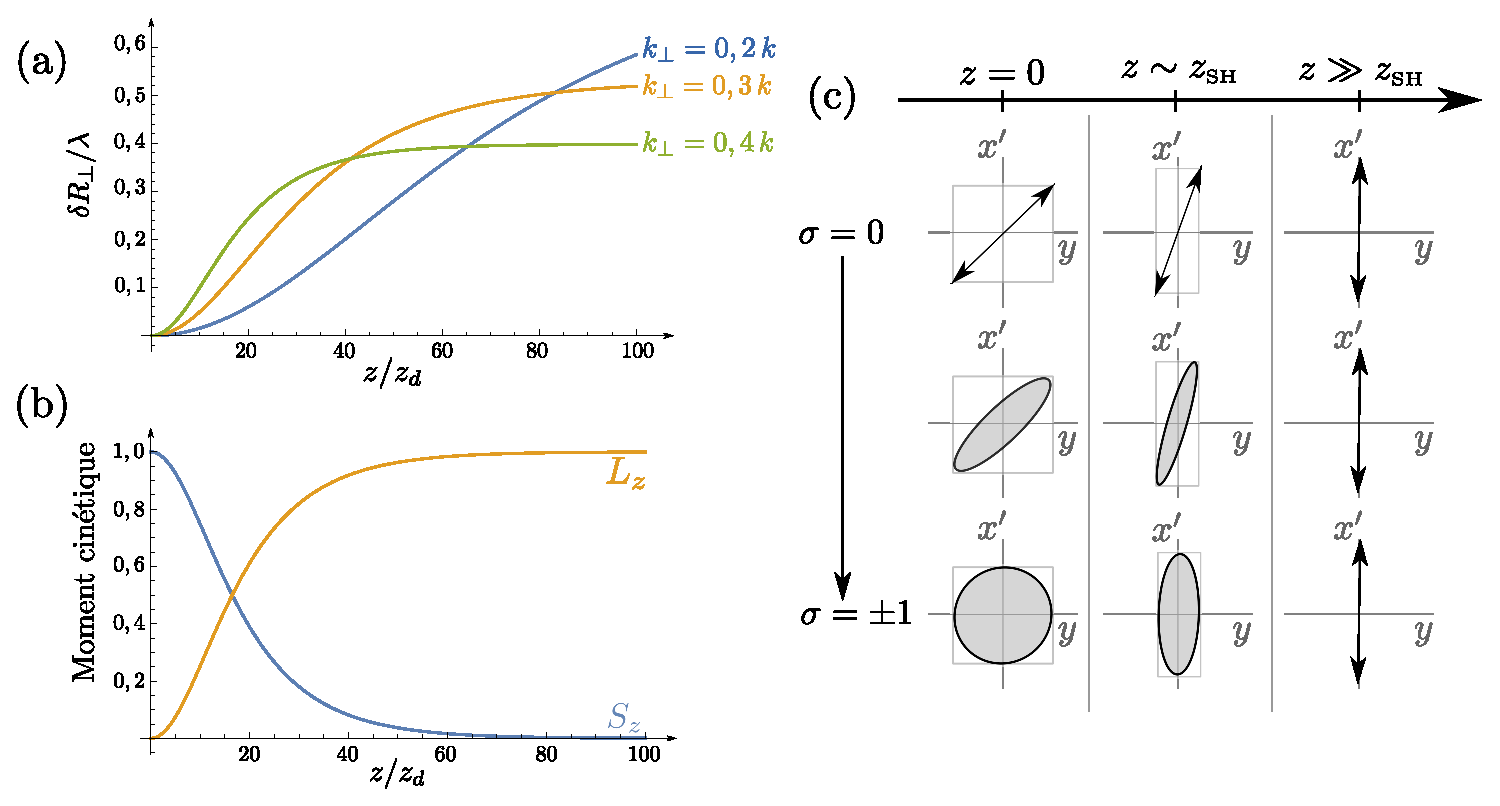
\includegraphics[width=\linewidth]{./Illustrations/Courbes.eps}
			\caption{(a) Graphe de l'évolution du déplacement $ \delta R_\perp $ en fonction de $ z $ pour différentes valeurs de l'angle d'incidence $k_\perp/k $ ; (b) Courbes des composantes $ S_z $ et $ L_z $ des moments cinétiques en fonction du temps $ z $ pour $ \sigma = + 1 $ et $ k_0 / k = 0,4 $. \`{A} l'instant initial, le système possède uniquement un moment cinétique de spin qui est converti au fur et à mesure de la propagation en moment cinétique orbital, la somme $ L_z + S_z $ restant constante ; (c) Schéma de l'évolution de la polarisation moyenne du faisceau au cours de la propagation dans le milieu désordonné.}
			\label{fig:Plot}
		\end{minipage}
	\end{figure}
	
	\subsubsection{\'Evolution du moment cinétique}
	\`A nouveau, en utilisant l'expression du champ électrique moyen, nous pouvons calculer l'expression des moments cinétiques du faisceau lumineux. Le moment cinétique orbital est alors donné par :
	\begin{equation*}
		\label{exp_L(z)}
		\vec{L}(z) = \left(\vec{R}_\perp(z) + z \, \vec{e}_z \right) \wedge ( \vec{k}_\perp + k_z \vec{e}_z ) 
	\end{equation*}
	où nous reconnaissons alors la forme classique bien connue $ \vec{L} = \vec{R} \wedge \vec{p} $ où $ \vec{p} = \vec{k}_0 + k_z \vec{e}_z $.\\
	
	Le spin est lui donné par l'expression :
	\begin{equation}
		\label{exp_S(z)}
		S_z(z) =  \frac{ \sigma}{ \cosh \left( z/z_\text{{\tiny SH}} \right) } \; .
	\end{equation}
	
	Leur évolution est alors tracée sur le graphe présenté figure \ref{fig:Plot}(b) pour une polarisation initiale circulaire. Nous voyons ainsi que le moment cinétique de spin diminue tandis que le moment orbital augmente (le moment cinétique total selon $ z $ reste lui constant car le milieu est statistiquement invariant par rotation autour de cet axe). Ce transfert de moment cinétique s'explique par une déformation de la polarisation du faisceau au fur et à mesure de la propagation dans le milieu désordonné comme schématisé sur la figure \ref{fig:Plot}(c). Nous voyons alors que la polarisation moyenne du faisceau tend vers une polarisation rectiligne (pour laquelle le spin est nul) ce qui explique la saturation du décalage que nous avions mis en évidence précédemment.
	
%	\begin{figure}[h]
%		\centering
%		\begin{minipage}[c]{0.85\linewidth}
%			\centering
%			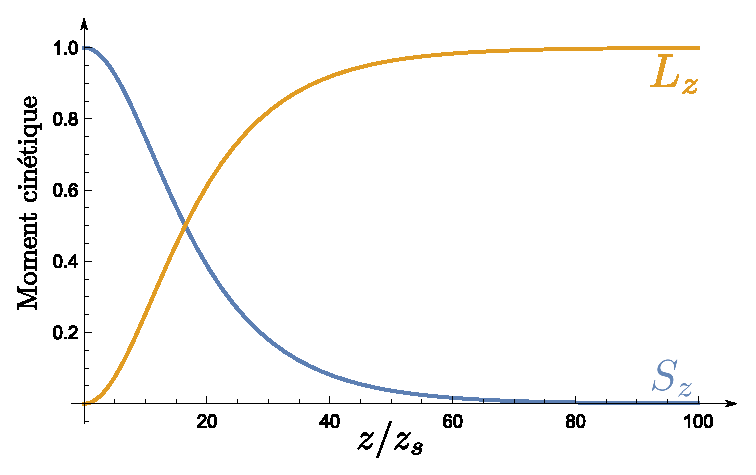
\includegraphics[width=0.7\linewidth]{./Illustrations/Plot_conversion_L-S.eps}
%			\caption{Courbes des composantes $ S_z $ et $ L_z $ des moments cinétiques en fonction du temps $ z $ pour $ \sigma = + 1 $ et $ k_0 / k = 0.4 $. \`{A} l'instant initial, le système possède uniquement un moment cinétique de spin qui est converti au fur et à mesure de la propagation en moment cinétique orbital, la somme $ L_z + R_z $ restant constante.}
%			\label{fig:conversion_moment_cinetique}
%		\end{minipage}
%	\end{figure}
	
	\section{Conclusion}
	
	Durant ma thèse, j'ai ainsi étudié l'effet Hall de spin dans le cas d'un désordre transverse. Nous avons montré que cette effet était résistant au moyennage sur les différentes configurations du désordre. De plus, en considérant ici l'aspect vectoriel de la lumière, nous avons mis en évidence l'effet du désordre sur l'état polarisation du faisceau.\\
	
	Un point intéressant de ma thèse est le travail sur l'analogie lumière-matière. De tels concepts peuvent être particulièrement pratiques pour proposer des illustrations aux élèves et tenter de mieux leur permettre d'appréhender des notions qui sont plus intuitives en optique ou inversement.
	
	
	\section{Enseignement et médiation scientifique}
	\subsection{Monitorat au sein de Sorbonne Université}
	Durant mes trois années de thèse, j'ai effectué un monitorat au sein de l'université Sorbonne Université. L'enseignement était déjà quelque chose qui me tenait à cœur avant cela, en effet, j'ai toujours considéré que la transmission des connaissances est une étape essentielle de l'apprentissage personnel. C'est pour cela qu'il était très important pour moi de pouvoir compléter mon travail de recherche au cours de ma thèse par des enseignements. Mon monitorat a confirmé ma vocation de professeure.\\ 
	
	J'ai encadré des groupes de travaux dirigés de mécanique en L2 pendant lesquels j'ai pû développer mes capacités de calculs au tableau et une approche pédagogique insistant sur l'importance pour les étudiant\pointmedian es de pouvoir poser des questions. J'y ai également appris à gérer mon planning, devant balancer la contrainte du programme (et des examens) avec un rythme permettant aux étudiant\pointmedian es de bien saisir les notions importantes et de s'approprier les outils vus en cours.\\
	
	J'ai également encadré des groupes de travaux pratiques d'optique. Ici, le format en demi-groupe et avec des binômes amenait à un encadrement plus proche et permettant de discuter plus en profondeur les notions physiques avec les étudiant\pointmedian es. Pendant ces séances, j'ai également dû gérer une évaluation continue des étudiant\pointmedian es par la correction de comptes-rendus ainsi que par la tenue d'interrogations rapides à chaque séance.\\
	
	\subsection{Participation au tournoi de physique}
	Au cours de mon cursus à Sorbonne Université j'ai pris part au \textit{French Physicists' Tournament} (qui constitue la sélection française de l'\textit{International Physicists' Tournament}). Durant celui-ci, des équipes, issues de différentes universités et écoles, se retrouvent pour \textgravedbl s'affronter\textacutedbl{} sur des problèmes de physique ludiques où elles doivent présenter et critiquer les résultats qu'elles ont obtenus durant un semestre de travail. Il s'agit d'un moment où ont lieu de nombreuses discussions physiques, ainsi qu'une première expérience du travail de recherche pour de nombreu\pointmedian ses étudiant\pointmedian es.\\
	
	J'ai tout d'abord participé en tant que membre de l'équipe durant ma première année de master. Comme pour beaucoup, cela a été pour moi l'une des premières occasions où j'ai pu étudier en très grande autonomie un sujet de physique, mais cela a surtout été une première expérience de présentation de mes résultats personnels et du travail d'un semestre entier sur un temps de 10 minutes. Pendant cette présentation, il fallait ainsi être pédagogique (le jury composé de physicien\pointmedian nes ne connaissant pas spécialement les sujets) et présenter correctement sa démarche et ses résultats tout en restant très concis.\\
	
	J'ai ensuite eu l'occasion durant mon monitorat d'encadrer l'équipe de Sorbonne Université. J'ai pu y transmettre ma propre expérience du tournoi, ainsi que de discuter avec des étudiant\pointmedian es en master du travail de recherche et de la démarche scientifique. L'encadrement de tels projets est très particulier, en effet, les étudiant\pointmedian es doivent construire leur propre démarche, et nous cherchions à leur donner le plus d'autonomie possible, il fallait donc accompagner les étudiant\pointmedian es et être prête à répondre à leurs questions sans essayer de les guider dans une direction particulière. Il s'agit aussi d'une expérience d'enseignement où il est nécessaire de jongler entre de nombreux domaines de la physique et sur des sujets que l'on ne maitrise pas entièrement au premier abord.\\
	
	\`A présent je participe à l'organisation de ce tournoi qui est également un grand moment de partage scientifique en tout genre. Il s'agit de réfléchir à la sélection des sujets pour le tournoi français, en équilibrant les divers domaines, mais également les types d'approches que les questions vont demander (expérience de coin de table, simulations, traitement de données, problème d'ingénierie, etc.). Il y a également de nombreuses questions de logistique à gérer. Tout cela demande évidemment un bon travail d'équipe et de répartition des tâches.\\ %En ce qui me concerne, j'ai été chargée pour l'année 2021 (où le tournoi s'est déroulé en distanciel) de comparer les options de visio-conférences disponibles. Pour l'année 2022, je me suis occupée des réservations de l'hôtel, il m'a donc fallu effectuer des demandes de devis et comparer les différentes offres.
	
	Ce genre d'événements est pour moi quelque chose de particulièrement enrichissant pour les élèves et j'espère pouvoir continuer à m'investir en tant que professeure dans des structures similaires telles que les Olympiades de physique.
	
	
	\subsection{Vulgarisation scientifique}
	Au cours de mon stage de M2, puis de ma thèse j'ai pu participer au stand du Laboratoire Kastler Brossel de la Fête de la Science sur le campus Pierre et Marie Curie. Au sein de celui-ci, nous présentions de nombreuses expériences autour de la lumière, allant d'une \textgravedbl simple\textacutedbl{} mesure de la vitesse de la lumière à la production d'un laser en passant par les phénomènes d'interférences, ainsi que la démonstration historique de Kastler sur l'absorption et l'émission du sodium. De plus, nous recevons des publics très variés allant de classes de primaire à des universitaires, cela m'a ainsi appris à adapter mon discours et ma pédagogie aux personnes en face de moi et en fonction de la difficulté des sujets. Nous devions également gérer des questions de temps soit dans le cas de groupes scolaires qui étaient sur un planning précis, soit car le laboratoire organisait également des visites qui partaient à intervalles réguliers du stand. Ayant participé à trois reprises à la Fête, je connaissais très bien le stand et je faisais partie de l'équipe de préparation et d'installation.\\
	
	Ce sont des expériences que j'aimerai pouvoir reproduire à l'échelle de mes classes voir d'un établissement en proposant à mes élèves de présenter des projets personnels devant un public d'autres élèves, de parents et de professeur\pointmedian es.
	
	\subsection{Autres activités}
	Durant mes années d'études à Sorbonne Université, j'ai également pris une part très active dans l'association des étudiant\pointmedian es de physique CurieOsity.\\ 
	Au sein de celle-ci, j'ai pu participé à l'organisation de séances de tutorat, durant lesquelles des étudiant\pointmedian es de licences voire de master pouvaient venir librement pour demander de l'aide sur certains sujets. Cela nous forçait en tant qu'encadrant\pointmedian es à devoir comprendre efficacement et en un temps court les différents sujets pour pouvoir les expliquer clairement, en s'adaptant au niveau de l'étudiant\pointmedian e concerné\pointmedian e. Cela nous obligeait ainsi également à avoir en tête les différents programmes de l'université.\\
	Nous organisions aussi des rencontres entre chercheur\pointmedian euses et étudiant\pointmedian es sous un format un peu informel appelé les \textit{cafés-prof} pendant lesquels les professeur\pointmedian es pouvaient présenter leur domaine de recherche mais également leur parcours. Nous avons également organisé des conférences plus traditionnelles.\\
	L'association était aussi une interlocutrice privilégiée des équipes pédagogiques de l'université. Nous étions ainsi contacté pour discuter des envies et des besoins des étudiant\pointmedian es, ou pour faire le pont avec l'administration dans certaines situations. En particulier, nous avions participé à l'élaboration de la nouvelle maquette du master.\\
	
	Je me suis également investie personnellement au sein des structures de l'université, tout d'abord pendant mon master au sein du conseil de l'UFR, puis en tant que représentante des doctorant\pointmedian es au conseil de l'école doctorale. Je compte également m'impliquer le plus possible dans les instances de mon futur établissement.
	
	
\end{document}
